\nomenclature[A]{ICT}{Information and Communication Technology}
\nomenclature[A]{ITS}{Intelligent Transportation System}
\nomenclature[A]{ATIS}{Advanced Traveler Information Systems}
\nomenclature[A]{ATMS}{Advanced Transportation Management Systems}
\nomenclature[A]{APTS}{Advanced Public Transportation Systems}
\nomenclature[A]{V2I}{Vehicle-to-Infrastructure}
\nomenclature[A]{V2V}{Vehicle-to-Vehicle}
\nomenclature[A]{GPS}{Global Positioning Systems}
\nomenclature[A]{DSRC}{Dedicated Short-Range Communications}
\nomenclature[A]{CACC}{Cooperative Adaptive Cruise Control}
\nomenclature[A]{ISO}{International Standards Organization}
\nomenclature[A]{BPM}{Burst Position Modulation}
\nomenclature[A]{FEC}{Forward error correction}
\nomenclature[A]{SECDED}{Single-Error-Correct-Double-Error-Detect}
\nomenclature[A]{RS}{Reed-Solomon}
\nomenclature[A]{PSR}{Preamble Symbol Repetitions}
\nomenclature[A]{DPS}{Dynamic Preamble Select}
\nomenclature[A]{SS-TWR}{Single-sided two-way ranging}
\nomenclature[A]{DS-TWR}{Double-sided two-way ranging}



In Section 2.1, we provide a background about Intelligent Transportation System (ITS). In Section 2.2 we discuss vehicle platooning concept and control functions. In Section 2.3, we describe the features of a vehicular RF channel. In Section 2.4, 2.5, and 2.6 we provide a short introduction on WiFi-p, UWB, and UWB ranging, respectively. In Section 2.7 and 2.8, we provide background about LPCXpresso4337 development board and DecaWave DW1000 UWB transceiver respectively. 

\section{Intelligent Transportation System}
It is envisioned that Information and Communication Technology (ICT) can increase the efficiency of the current transportation system significantly. This will require a significant investment because embedding transportation systems with sensors, wireless communication technologies, and other electronics will be needed to make them more intelligent. Hence the name Intelligent Transportation System (ITS). According to \cite{ezell2010explaining}, ITS applications can bring benefits such as increasing driver and pedestrian safety \cite{facts2008data}, performance improvement of the transportation network, enhanced convenience \cite{drane1998positioning}, delivering environmental benefits, and boosting productivity, economic, and employment growth. ITS enables a broad range of ITS applications such as Advanced Traveler Information Systems (ATIS), Advanced Transportation Management Systems (ATMS), ITS-Enabled Transportation Pricing Systems, Advanced Public Transportation Systems (APTS), Vehicle-to-Infrastructure (V2I) and Vehicle-to-Vehicle (V2V) integration. To support the diverse array of applications, a wide range of technologies are combined by ITS such as Global Positioning Systems (GPS) \cite{el2002introduction}, cellular technology, Dedicated Short-Range Communications (DSRC), camera recognition, etc.

\section{Vehicle Platooning}
Vehicle platooning is a concept that aims to increase the current road capacity. The key in achieving this goal is the organization of vehicles in tightly controlled groups, also called platoons that operate close together. Several implementations of vehicle platooning concept have been proposed. Some potential implementations of vehicle platooning are described below \cite{vugts2010string}:

\subsubsection{Adaptive Cruise Control(ACC)}
Figure \ref{fig:Vehicle Platoon using ACC} illustrates a three-vehicle platoon using ACC. Front radar of an ACC system is only able to detect vehicles in line of sight. ACC system is not able to measure the distance and speed of the vehicle driving in front of the immediately preceding vehicle or behind the vehicle or in a different lane as shown in Figure \ref{fig:A typical view of a front-radar used in ACC}. Moreover, speed information flows down the platoons with increasing delays potentially leading to unstable platoons and unsafe traffic. To overcome these shortcomings, Cooperative Adaptive Cruise Control (CACC) is implemented in platoons. 

\begin{figure}[h!]
    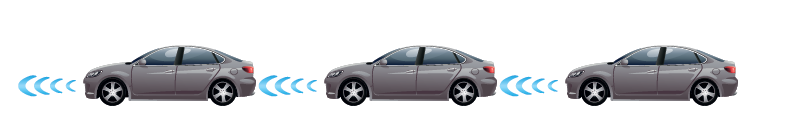
\includegraphics[width=1\textwidth]{figures/vehiclePlatoonusingACC.png}
    \centering
    \caption{Vehicle platoon using ACC}
    \label{fig:Vehicle Platoon using ACC}    
\end{figure}

\begin{figure}[h!]
    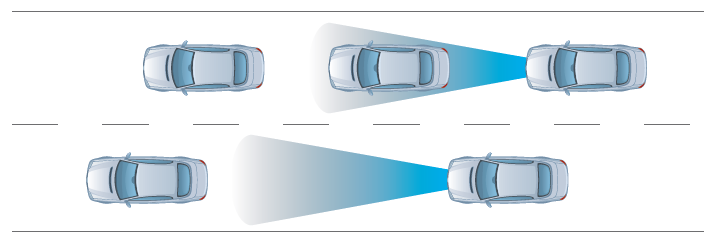
\includegraphics[width=1\textwidth]{figures/typicalviewoffrontradarusingACC.png}
    \centering
    \caption{A typical view of a front-radar used in ACC}
    \label{fig:A typical view of a front-radar used in ACC}    
\end{figure}

\begin{figure}[h!]
    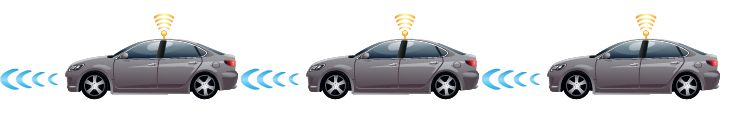
\includegraphics[width=1\textwidth]{figures/vehicleplatooningusingCACC.png}
    \centering
    \caption{Vehicle platoon using CACC}
    \label{fig:vehicleplatooningusingCACC}    
\end{figure}

\subsubsection{Cooperative Adaptive Cruise Control}
CACC augments ACC with wireless communication, new control logic and GPS as illustrated in Figure \ref{fig:vehicleplatooningusingCACC}. Wireless communication allows vehicles to extend their view beyond the LOS of the radar. With CACC, the third vehicle in the illustration of Figure \ref{fig:vehicleplatooningusingCACC} is notified via wireless communication of the behavior of the leading vehicle. The third vehicle can almost instantly react to speed changes of the first vehicle and as a result, a CACC system enables to drive with closer headways.

\subsubsection{Automated Highway System (AHS)}
With both ACC and CACC, the driver is (partly) responsible for the operation of the vehicle. The driver is for example still responsible for steering the vehicle. The next step in vehicle platooning is a system in which vehicles are fully automated. AHS platoons are similar to CACC platoon as illustrated in Figure \ref{fig:vehicleplatooningusingCACC}. However, AHS platoons rely heavily on wireless communication to create automated and high cooperative vehicles.

\subsubsection{Advantages and Risks of Platooning}
The advantages of vehicle platooning include \cite{de1997behavioral} an increase in road capacity, reduction of environmental impacts, improved safety, improved driver comfort, highly cooperative groups, decrease in fuel consumption (reduced air resistance), shorter commutes during peak periods, etc. 

The risks of platooning include the driver is less in control being at the hands of computer software or lead driver and the driver is inattentive than usual hence not able to react as quickly to adverse situations if software or hardware fails.

\subsubsection{Vehicle Platooning Control Functions}
The most basic functionality for automated vehicles in vehicle platoons, being respectively longitudinal control, lateral control and maneuver control \cite{shladover2005automated}.

Longitudinal control of a vehicle is the feature that controls the speed and distance to the preceding vehicle using powertrain and brakes. Implementations of the longitudinal control rely heavily on measurements of headway and the speed of the preceding vehicle. Longitudinal controllers that control the speed of a vehicle, purely based on the vehicle's sensors are classified as autonomous. Autonomous controllers are capable of maintaining string stability i.e. headway errors do not flow down the platoon, under constant time gaps between vehicles. Another type of longitudinal control is cooperative control. These controllers typically complement radar and image-processing sensors with wireless communication to collect state information (position, speed, acceleration, and maneuver information) of close operating vehicles. These type of controllers are not only able to maintain string stability under constant time gap, like autonomous controllers, but also under constant distance gaps.

The primary functionality of lateral control is keeping the vehicle in the center of the lane. Lateral control is also concerned with lane changing wherein lane changing is the feature to steer a vehicle from the current lane to an adjacent lane.

Vehicle platooning involves, apart from longitudinal and lateral control, the coordination of vehicle maneuvers. These maneuvers are typically the formation and splitting of platoons, the merging of traffic streams and coordination of changing lanes.\\

Additional details on platooning and its implementation can be obtained by referring to SARTRE Report on Fuel Consumption, SARTRE Report on Infrastructure and Environment, \cite{bergenhem2010challenges}, \cite{chan2012cooperative}, \cite{davila2010sartre}, etc.

\section{Vehicular RF Channel} 
Key characteristics of vehicular channels are shadowing by other vehicles, high Doppler shifts, and inherent non-stationarity \cite{mecklenbrauker2011vehicular}. All have a major impact on the data packet transmission reliability and latency. For vehicular channels, it is customary to distinguish between V2V and V2I channels. These channels not only
differ from each other but also deviate significantly from those in cellular communication. In cellular scenarios, the base station (BS) is fixed, elevated, and located at or above rooftop level, such that its close surroundings are free of scatterers. Furthermore, most of the relevant scatterers are
immobile or move relatively slowly. The distance between the BS and the user span roughly from 10 m to 10 km. In a V2V communication scenario, there is neither an access point (AP) nor BS and both the Rx and the Tx may move with high velocities. The antennas are mounted at a the height of 1-2 m, many relevant scatterers (i.e., vehicles) move, and the distances between the Tx, the Rx, and principal scatterers are in the range of a few hundred meters. Depending on whether the scenario includes a the road in an open field or a busy street in an urban environment, the number of relevant scatterers might vary significantly.

The following five properties mainly characterize wireless channels.
\begin{itemize}
    \item Pathloss: How does the average received power level vary with distance to the transmitter?
    \item Signal fading: How does the instantaneous signal level fluctuate over time, frequency, and space?
    \item Delay spread: How is the signal smeared in time by echoes?
    \item Doppler spread: How is the transmitted signal smeared in frequency due to movements of the Rx, the Tx, and scatterers?
    \item Angular spread: How is the transmitted signal smeared over directions by antennas and scatterers?
\end{itemize}

The propagation conditions in particular for V2V communications
are influenced by the antennas and their placement on the vehicle. The roof of the vehicle can strongly affect the antenna pattern; if the antenna is placed on a backward-slanted roof, it has difficulties seeing vehicles in front of it.

The region over which the transmitter provides coverage is smaller than the area in which it creates interference. Due to high speeds involved, V2V channels show substantial time variance (the channel state changes) and non-stationarity (the channel statistics change). These effects are more pronounced for cars approaching each other or approaching intersections, while they are less severe for vehicles driving in convoys or V2I communications.

\section{WiFi-p}
An international standard, IEEE 802.11p \cite{ieee1997wireless}, which is part of the WAVE initiative, has gained considerable importance. Based on popular WiFi standard, it is intended for both V2I and V2V traffic telematics applications and operates in the 5.9-GHz band. Its importance is further highlighted by the European decision on the use of the 5875-5905 MHz frequency band for safety-related ITS applications \cite{reding2007commission}. IEEE 802.11p is an amendment to the IEEE 802.11 standard for vehicular networks. Modifications to the original standard were needed as the MAC, and PHY layers were never designed for mobile environments. We note that a 700 MHz band is devoted to advanced driving safety support systems in Japan \cite{mecklenbrauker2011vehicular}. IEEE 802.11p is also one mode of communication access for land mobiles, a framework for heterogeneous packet-switched communication in mobile environments approved by the International Standards Organization (ISO). Summarizing, the IEEE 802.11p standard has established itself as the key technology for V2V and safety-critical V2I communications.

Figure \ref{fig:DSRC spectrum band and channels} shows the DSRC spectrum band and its channels as allocated by the FCC. This allocation consists of 7 channels with a bandwidth of 10 MHz each. Some of these channels are restricted to be used for the transmission of a particular type of information. For instance, channel 178 is the control channel and can only be utilized for the transmission of safety-related data. The outer channels number 172 and 184 are reserved for special purpose communication, and the remaining four channels can be used for both safety and non-safety related communication \cite{chen2009ieee}.


\begin{figure}[h!]
    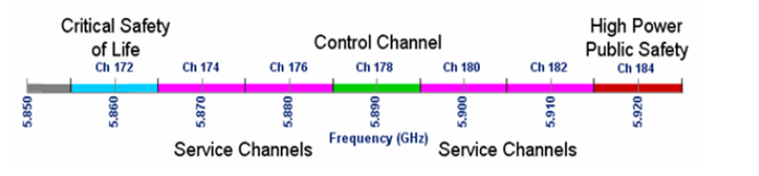
\includegraphics[width=1\textwidth]{figures/DSRC spectrum band and channels.png}
    \centering
    \caption[DSRC spectrum band and channels]{DSRC spectrum band and channels \protect\cite{chen2009ieee}}
%    \protect\citeA{chen2009ieee}
    \label{fig:DSRC spectrum band and channels}    
\end{figure}



\section{UWB}
UWB differs substantially from conventional narrowband radio frequency (RF) and spread spectrum technologies (SS), such as Bluetooth Technology and 802.11 a/g. UWB uses an extremely wide band of RF spectrum to transmit data as shown in Figure \ref{fig:Comparision of narrowband, spread spectrum, and ultra-wideband signal concepts}.

\begin{figure}[h!]
    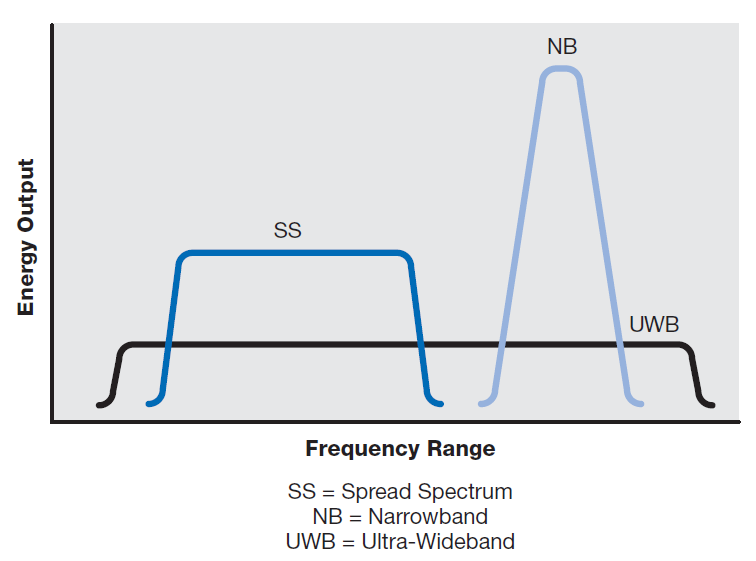
\includegraphics[width=0.7\textwidth]{figures/UWBcomparedtoNB.png}
    \centering
    \caption[Comparision of narrowband, spread spectrum, and ultra-wideband signal concepts]{Comparision of narrowband, spread spectrum, and ultra-wideband signal concepts   \protect \cite{IntelUWB}}
 
    
    \label{fig:Comparision of narrowband, spread spectrum, and ultra-wideband signal concepts}    
\end{figure}

The potential data rate over a given RF link is proportional to the bandwidth of the channel and the logarithm of the signal-to-noise ratio (Shannon’s Law) \cite{haykin2008communication}. RF design engineers typically have little control over the bandwidth parameter, because this is dictated by FCC regulations that stipulate the allowable bandwidth of the signal for a given radio type and application. Bluetooth technology, 802.11a/g Wi-Fi, cordless phones, and numerous other devices are relegated to the unlicensed frequency bands that are provided at 900 MHz, 2.4 GHz, and 5.1 GHz. Each radio channel is constrained to occupy only a narrow band of frequencies, relative to what is allowed for UWB.

UWB is a unique and new usage of a recently legalized frequency spectrum. UWB radios can use frequencies from 3.1 GHz to 10.6 GHz - a band more than 7 GHz wide. Each radio channel can have a bandwidth of more than 500 MHz, depending on its center frequency. To allow for such a large signal bandwidth, the FCC put in place severe broadcast power restrictions. By doing so, UWB devices can make use of an extremely wide frequency band while not emitting enough energy to be noticed by narrower band devices nearby, such as 802.11a/g radios \cite{karapistoli2010overview}. Figure \ref{fig:IEEE 802.15.4a UWB Frequency Bands} denotes the center frequencies and bandwidths of the defined bands, as well as the regulatory domains in which they are admissible. Frequency bands (channel numbers) 4, 7, 11, 15 have the same center frequency as bands 2, 5, 9, 13 respectively. This is due to the fact that bands 4, 7, 11, 15 are all "wide-band" channels whose bandwidth is larger than 1 GHz, and these bands, in fact, overlay the other 500 MHz wide bands.

\begin{figure}[h!]
    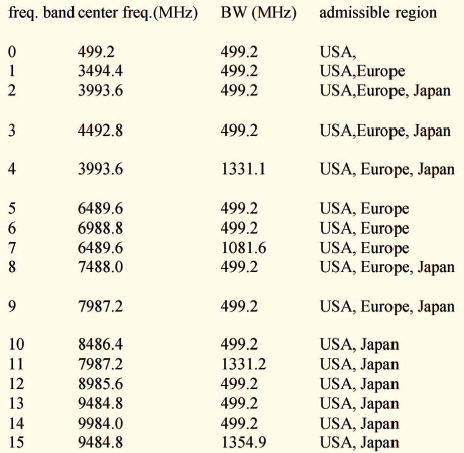
\includegraphics[width=0.8\textwidth]{figures/uwbchannels.png}
    \centering
   \caption[IEEE 802.15.4a UWB Frequency Bands]{IEEE 802.15.4a UWB Frequency Bands \protect\cite{zhang2009uwb}}
%    \protect\citeA{zhang2009uwb}
    \label{fig:IEEE 802.15.4a UWB Frequency Bands}    
\end{figure}

UWB communications are based on the transmission and reception of frames. Figure \ref{fig:UWB PHY Frame structure} shows the general structure of the UWB frame. It begins with a synchronization header consisting of the preamble and the Start of the Frame Delimiter (SFD), after which the PHY header (PHR) defines the length (and data rate) of the data payload part of the frame.

\begin{figure}[h!]
    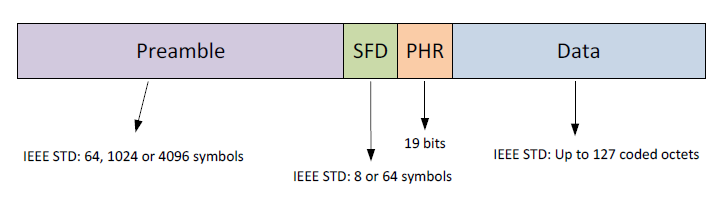
\includegraphics[width=0.8\textwidth]{figures/UWBPHYFrameStructure.png}
    \centering
    \caption[UWB PHY Frame structure]{UWB PHY Frame structure \protect\cite{DW1000UserManual}}
%    \protect\citeA{DW1000UserManual}
    \label{fig:UWB PHY Frame structure}    
\end{figure}

\begin{figure}[h!]
    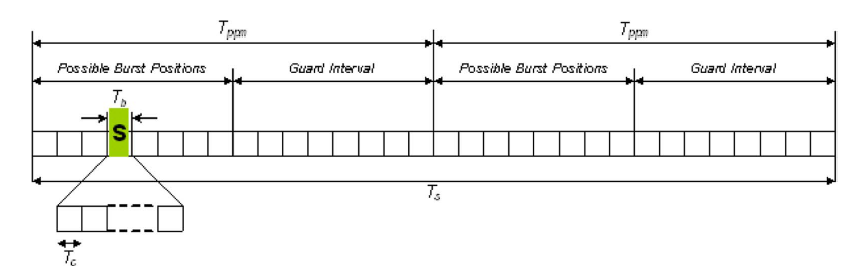
\includegraphics[width=0.8\textwidth]{figures/ModulationandTimehoppingof802.15.4a.png}
    \centering
    \caption[UWB Symbol duration]{UWB Symbol duration \protect\cite{gutierrez2004low}}
%    \protect\citeA{gutierrez2004low}
    \label{fig:UWB Symbol duration}    
\end{figure}

Figure \ref{fig:UWB Symbol duration} shows the UWB Symbol duration, $T_c$ is the chip (pulse) duration of approximately 2 ns, $T_b$ is the burst-hopping duration, which equals, $T_b$ = N$T_c$ = 32 ns, n indexes the N=16 pulses that are transmitted during each data burst. $T_{ppm}$ is the modulation interval for the pulse position modulation $T_{ppm}$ = 16$T_b$, and $T_s$ is the symbol duration.

The UWB used in 802.15.4 is also called impulse radio UWB because it is based on high-speed pulses of RF energy. During the PHR and data parts of the frame, information bits are signaled by the position of the burst, in a modulation scheme termed Burst Position Modulation (BPM). Each data bit passes through a convolution encoder to generate a "parity bit" used to set the phase of the burst as either positive or negative, this component of the modulation is termed binary phase-shift keying (BPSK). 

Also, the quarter symbol interval is sub-divided into 2, 4, or 8 sub-intervals and a pseudo random sequence used to determine both the burst shape and which of the sub-intervals are used for the burst transmission. This gives more immunity to interference and whitens the output spectrum allowing a higher signal power to be utilized in the transmitter.


To ensure that the signals can still be decoded by noncoherent receivers, a systematic code is used wherein the systematic code is one in which the information bits are transmitted unchanged along with the parity check bits. The systematic bits are used to determine the PPM position of the burst and are visible to both noncoherent and coherent receivers. The parity bits are modulated onto the burst phase and are thus visible only to coherent receivers. Forward error correction (FEC) is also included in the PHR and data parts of the frame. The 19-bit PHR includes a 6-bit Single-Error-Correct-Double-Error-Detect (SECDED) code and the data part of the frame has a Reed-Solomon (RS) code applied. Both SECDED and RS codes are systematic \cite{zhang2009uwb}.

The synchronization header consists of the preamble sequence and the SFD. In contrast to the BPM/BPSK modulation used for the PHR and data, the synchronization header is made up of single pulses. The symbol is divided into approximately 500 "chip" time intervals, (496/508 depending on 16/64 MHz PRF), in which either a negative or a positive pulse may be sent, or no pulse. The "chip" interval is 499.2 MHz, a fundamental frequency within the UWB PHY, and so the resultant symbol times are thus 496/499.2 us for 16 MHz PRF, 508/499.2 us for 64 MHz PRF. It is to be noted that number of chips per burst change for PRF of 16 or 64 MHz. The number of chips per burst for 64 MHz PRF will be four times greater than the number of chips per burst for 16 MHz PRF  \cite{gutierrez2004low}.

The sequence of pulses sent during the symbol interval is determined by preamble code. The standard defines eight different length-31 preamble codes for use at 16 MHz PRF and 16 different length-127 preamble codes for use at 64 MHz PRF. 

The standard nominates particular codes for specific channels so that at 16 MHz PRF there are just two to choose from per channel, while at 64 MHz PRF there is a choice of four codes per channel. The length-31 codes are spread by inserting 15 zeros for each code point to give the 496 chip times per symbol while the length-127 codes are spread by adding three zeros for each code point to give the 508 chip times per symbol. The preamble length is defined by how many times (i.e. for how many symbols) the sequence is repeated. This is determined by the configuration of Preamble Symbol Repetitions (PSR).

The standard defines PSR settings of 16, 64, 1024 and 4096. The preamble sequence has a property of perfect periodic autocorrelation \cite{ipatov1979ternary} which in essence allows a coherent receiver to determine the exact impulse response of the RF channel between transmitter and receiver. This brings two significant benefits. Firstly, it allows the receiver to make use of the received energy from multiple paths, turning multipath from an interference source into a positive affect extending operating range. Secondly, it lets the receiver resolve the channel in detail and determine the arrival time of the first (most direct) path, even when attenuated, which brings precision advantages for Real Time Location System (RTLS) applications. 
The SFD marks the end of the preamble and the precise start of the switch into the BPM/BPSK modulation of the PHR. The time-stamping of this event is very deterministic in terms of symbol times, and it is this in conjunction with determining the first arriving ray within that symbol time that allows the accurate time-stamping needed for precision RTLS applications.

The standard specifies the SFD, which consists of the preamble symbols either not sent, or sent as normal or sent inverted (i.e. positive and negative pulses reversed) in a defined pattern eight symbol times long for data rates other than 110 kbps, and 64 symbols long for the 110 kbps mode.

The PHY header (PHR) is modulated using the BPM/BPSK modulation scheme, but it does not employ the Reed-Solomon code used for data, instead is employs a 6-bit SECDED parity check sequence as part of its 19-bit length.

The preamble codes specified by the standard for use on a particular channel were chosen to have a low cross-correlation factor with each other with the intention that the complex channels could operate independently from each other as separate networks.

The IEEE 802.15.4 UWB PHY standard includes a feature called Dynamic Preamble Select (DPS) intended for use in a security mechanism for two-way ranging, where devices switch to using one of the DPS specific preamble codes for the ranging exchange, and perhaps a different one for each direction of communication. The idea is to make it harder to eavesdrop or spoof, by randomly changing the DPS preamble codes in a mutually agreed sequence only known to the valid participants.


\section{UWB Ranging}
In all of the schemes that follow one node acts as Initiator, initiating a range measurement, while the other node acts as a Responder listening and responding to the initiator, and calculating the range. 

Single-sided two-way ranging (SS-TWR) involves a simple measurement of the round trip delay of a single message from one node to another, and a response sent back to the original node. 

\begin{figure}[h!]
    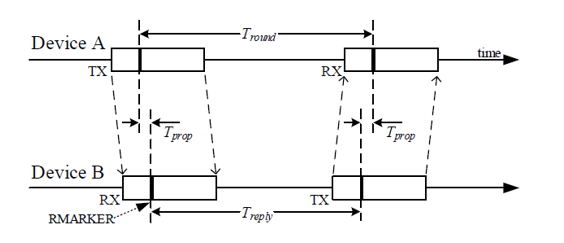
\includegraphics[width=0.8\textwidth]{figures/SSTWR.png}
    \centering
    \caption[Single-sided Two-way ranging]{Single-sided Two-way ranging \protect\cite{DW1000UserManual}}
%    \cite{DW1000UserManual}
    \label{fig:Single-sided Two-way ranging}    
\end{figure}

The operation of SS-TWR is as shown in Figure \ref{fig:Single-sided Two-way ranging}, where device A initiates the exchange and device B responds to complete the exchange and each device precisely timestamps the transmission and reception times of the message frames, and so can calculate times $T_{round}$ and $T_{reply}$ by simple subtraction.  And the resultant time-of-flight, $T_{prop}$ may be estimated by the equation:  
\begin{equation}
 T_{prop} = 0.5 (T_{round} - T_{reply})
\end{equation}

The times $T_{round}$ and $T_{reply}$ are measured independently by device A and B using their respective local clocks, wherein both have some clock offset error eA and eB from their nominal frequency, and so the resulting time-of-flight estimate has a considerable error that increases as $T_{reply}$ increases.  Depending on the size of ranging error that is acceptable to the application, SS-TWR may be an appropriate choice for range measurement especially if the reply time $T_{reply}$ is minimized and the clock error is low.  It should be noted that the reply time $T_{reply}$ is not just the RX-to-TX turnaround time but also includes the message length. 

It can be seen that as $T_{reply}$ increases and as the clock offset increases the error in the time-of-flight estimation increases to the point where the error is such as to render the estimation very inaccurate.  For this reason, SS-TWR is not commonly used, but it is worthy of examination for particular use cases where tight tolerance clocks are used, and the communication range is relatively short \cite{gutierrez2004low}.

Double-sided two-way ranging (DS-TWR), is an extension of the basic single-sided two-way ranging in which two round trip time measurements are used and combined to give a time-of-flight result which has a reduced error even for quite long response delays.  The operation of DS-TWR is as shown in Figure \ref{fig:Double-sided Two-way ranging}, where device A initiates the first round trip measurement to which device B responds, after which device B starts the second round trip measurement to which device A responds completing the full DS-TWR exchange.  Each device precisely timestamps the transmission and reception times of the messages. The four messages of DS-TWR, shown in Figure \ref{fig:Double-sided Two-way ranging}, can be reduced to three messages by using the reply of the first round-trip measurement as the initiator of the second round-trip measurement. The resultant time-of-flight estimate, $T_{prop}$, in both the three and four message cases may be calculated using the expression: 
\begin{equation}
T_{prop}=(T_{round1} \times T_{round2}-T_{reply1} \times T_{reply2})/(T_{round1}+T_{round2}+T_{reply1}+T_{reply2})
\end{equation}



\begin{figure}[h!]
    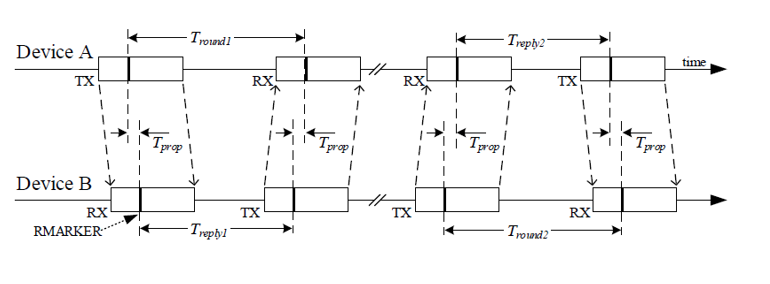
\includegraphics[width=0.8\textwidth]{figures/DSTWR.png}
    \centering
    \caption[Double-sided Two-way ranging]{Double-sided Two-way ranging \protect\cite{DW1000UserManual}}
%    \cite{DW1000UserManual}
    \label{fig:Double-sided Two-way ranging}    
\end{figure}

Both of the above schemes are denoted ASYMMETRIC because they do not require the reply times from each device to be the same.   
Using this scheme, the typical clock induced error is in the low picosecond range even with 20 ppm crystals. At these error levels, the precision of determining the arrival time of the messages at each of the receivers is a more significant contributor to overall $T_{prop}$ error than the clock-induced error. 

There is a special case of the double sided scheme known as SYMMETRIC Double-sided Two-way ranging in which $T_{reply1}$ and $T_{reply2}$ are restrained to be equal (or as close to equal as possible).  In this case: 

\begin{equation}
T_{prop}=(T_{round1} - T_{reply2} + T_{round2} + T_{reply1})/4
\end{equation}

This scheme requires only addition, subtraction, and division by four which is easily achieved in low power microcontrollers however it results in the entire exchange taking longer than necessary. 

The sources of error for ranging include Clock drift, Frequency drift, $T_{reply}$ (turnaround time from receiver to transmitter or vice versa, including the time required for creation of message), ranging transaction performed while one of the devices is transitioning through the crystal warm-up phase (during duty cycling) and bias which varies with received signal strength.

\section{LPCXpresso4337 development board}
The LPCXpresso4337 board {\cite{LPCUserManual}} has been developed by NXP to enable evaluation of and prototyping with the LPC4300 family of MCUs and features the LPC4337 in its 100 PIN BGA package option. LPCXpresso is a low-cost development platform available from NXP supporting NXP's ARM-based microcontrollers. The platform is comprised of a simplified Eclipse-based IDE and low-cost target boards which include an attached SWD debugger. LPC4337 has a dual core (M4 and M0) MCU running at up to 208 MHz. It includes up to 264 KB of SRAM. 
The LPCXpresso4337 board includes the following features: 
\begin{itemize}
    \item On-board, high-speed USB based, Link2 debug probe with support for ARM’s CMSIS-DAP, LPCXpresso IDE Redlink and SEGGER J-Link protocol options 
    \item Link2 probe can be used with on-board Target MCU or external target 
    \item Support for external debug probes 
    \item Tri-color LED 
    \item Target Reset, ISP and WAKE buttons 
    \item Expansion options based on Arduino UNO and PMod, plus additional expansion port pins 
    \item UART, I2C, and SPI port bridging from Target MCU to USB via the on-board debug probe 
    \item UART connector 
\end{itemize}

More information about the peripherals available on the chip can be found in the user manual \cite{LPCUserManual}.

\section{DecaWave DW1000}
DW1000 \cite{DW1000UserManual} is an IEEE 802.15.4-2011 UWB compliant wireless transceiver module. Its features include high data rate communications, low power consumption, small physical size, highly immune to fading, etc. The DecaWave DW1000 transceiver is embedded on to the LPCXpresso4337 board. It spans 6 RF bands from 3.5 GHz to 6.5 GHz and supports data rates of 110 kbps, 850 kbps, and 6.8 Mbps.

The DW1000 consists of an analog front-end (both RF and baseband) containing a receiver and transmitter and a digital backend that interfaces to a host processor, controls the analog front-end, accepts data from the host processor for transmission and provides received data to the host processor over an industry standard SPI interface. 

The DW1000 provides capabilities to take accurate transmission timestamp, supports delayed transmission, extended length data frames, cyclic redundancy check, frame filtering, automatic acknowledgment, automatic receiver re-enable, etc.

DW1000 supports Smart transmit power control. The power output regulations typically specify limits as -41 dBm in each 1 MHz bandwidth and generally measure this using a 1 ms dwell time in each 1 MHz segment.  When sending short frames at 6.8 Mbps, it is possible for a single frame to be transmitted in a fraction of a millisecond. So long as the transmitter does not transmit again within that same millisecond, the power of that transmission can be increased while complying with the regulations.  This power increase will increase the transmission range. Smart TX power control acts at the 6.8 Mbps data rate. DW1000 allows operating using different channels, preamble codes, preamble lengths, with Standard SFD or non-standard SFD, PRF, etc.

More information about DW1000 can be found in the datasheet \cite{DW1000DataSheet} and user manual \cite{DW1000UserManual}.